\section{Vista Lógica}\label{sec:vista-logica}

La Vista Lógica describe la arquitectura lógica de la plataforma, utilizando varios niveles de refinamiento. En particular, se presentan y describen los principales componentes lógicos de la plataforma así como sus responsabilidades, dependencias e interacciones. Se utilizan Diagramas de Componentes UML \cite{Ambysoft2018b}, con el clasificador \enquote{subsystem} para la arquitectura general y \enquote{component} para los refinamientos.

\subsection{Arquitectura General del Sistema}

La plataforma se descompone en dos subsistemas principales: el Componente Móvil, utilizado por los choferes, y el Componente Central, que concentra el resto de las funcionalidades y se comunica con los nodos periféricos y los sistemas externos (Figura \ref{fig:vista_logica}).

El Componente Central se organiza en capas. La capa de presentación está formada por la API REST, consumida por el componente móvil, el Frontoffice, para el público, los ciudadanos y los funcionarios, y el Backoffice de autoridades y administradores. La capa de servicios y procesamiento agrupa los Servicios de Negocio (autorización, empresas, vehículos, viajes y casos), la Generación de Reportes, la Ingesta de Eventos y el Motor de Fiscalización, que es disparado por la ingesta para detectar incumplimientos de forma asincrónica. La Persistencia almacena los datos declarados, los eventos, los casos y la pista de auditoría. Finalmente, la capa de adaptadores e infraestructura aísla la integración con Usuario gub.uy (OpenID Connect), la PDI (SOAP), el servicio de correo (SMTP), el nodo de Balanzas (solicitud--respuesta) y el nodo de Tracking, cuyos eventos llegan de forma asincrónica mediante el subsistema de Mensajería.

El Componente Móvil cuenta con su propia persistencia local, donde mantiene la Guía descargada, el estado del viaje y la cola de eventos pendientes, lo que le permite operar sin conectividad y sincronizar con el Componente Central mediante REST sobre HTTPS.

\begin{figure}[H]
    \centering
    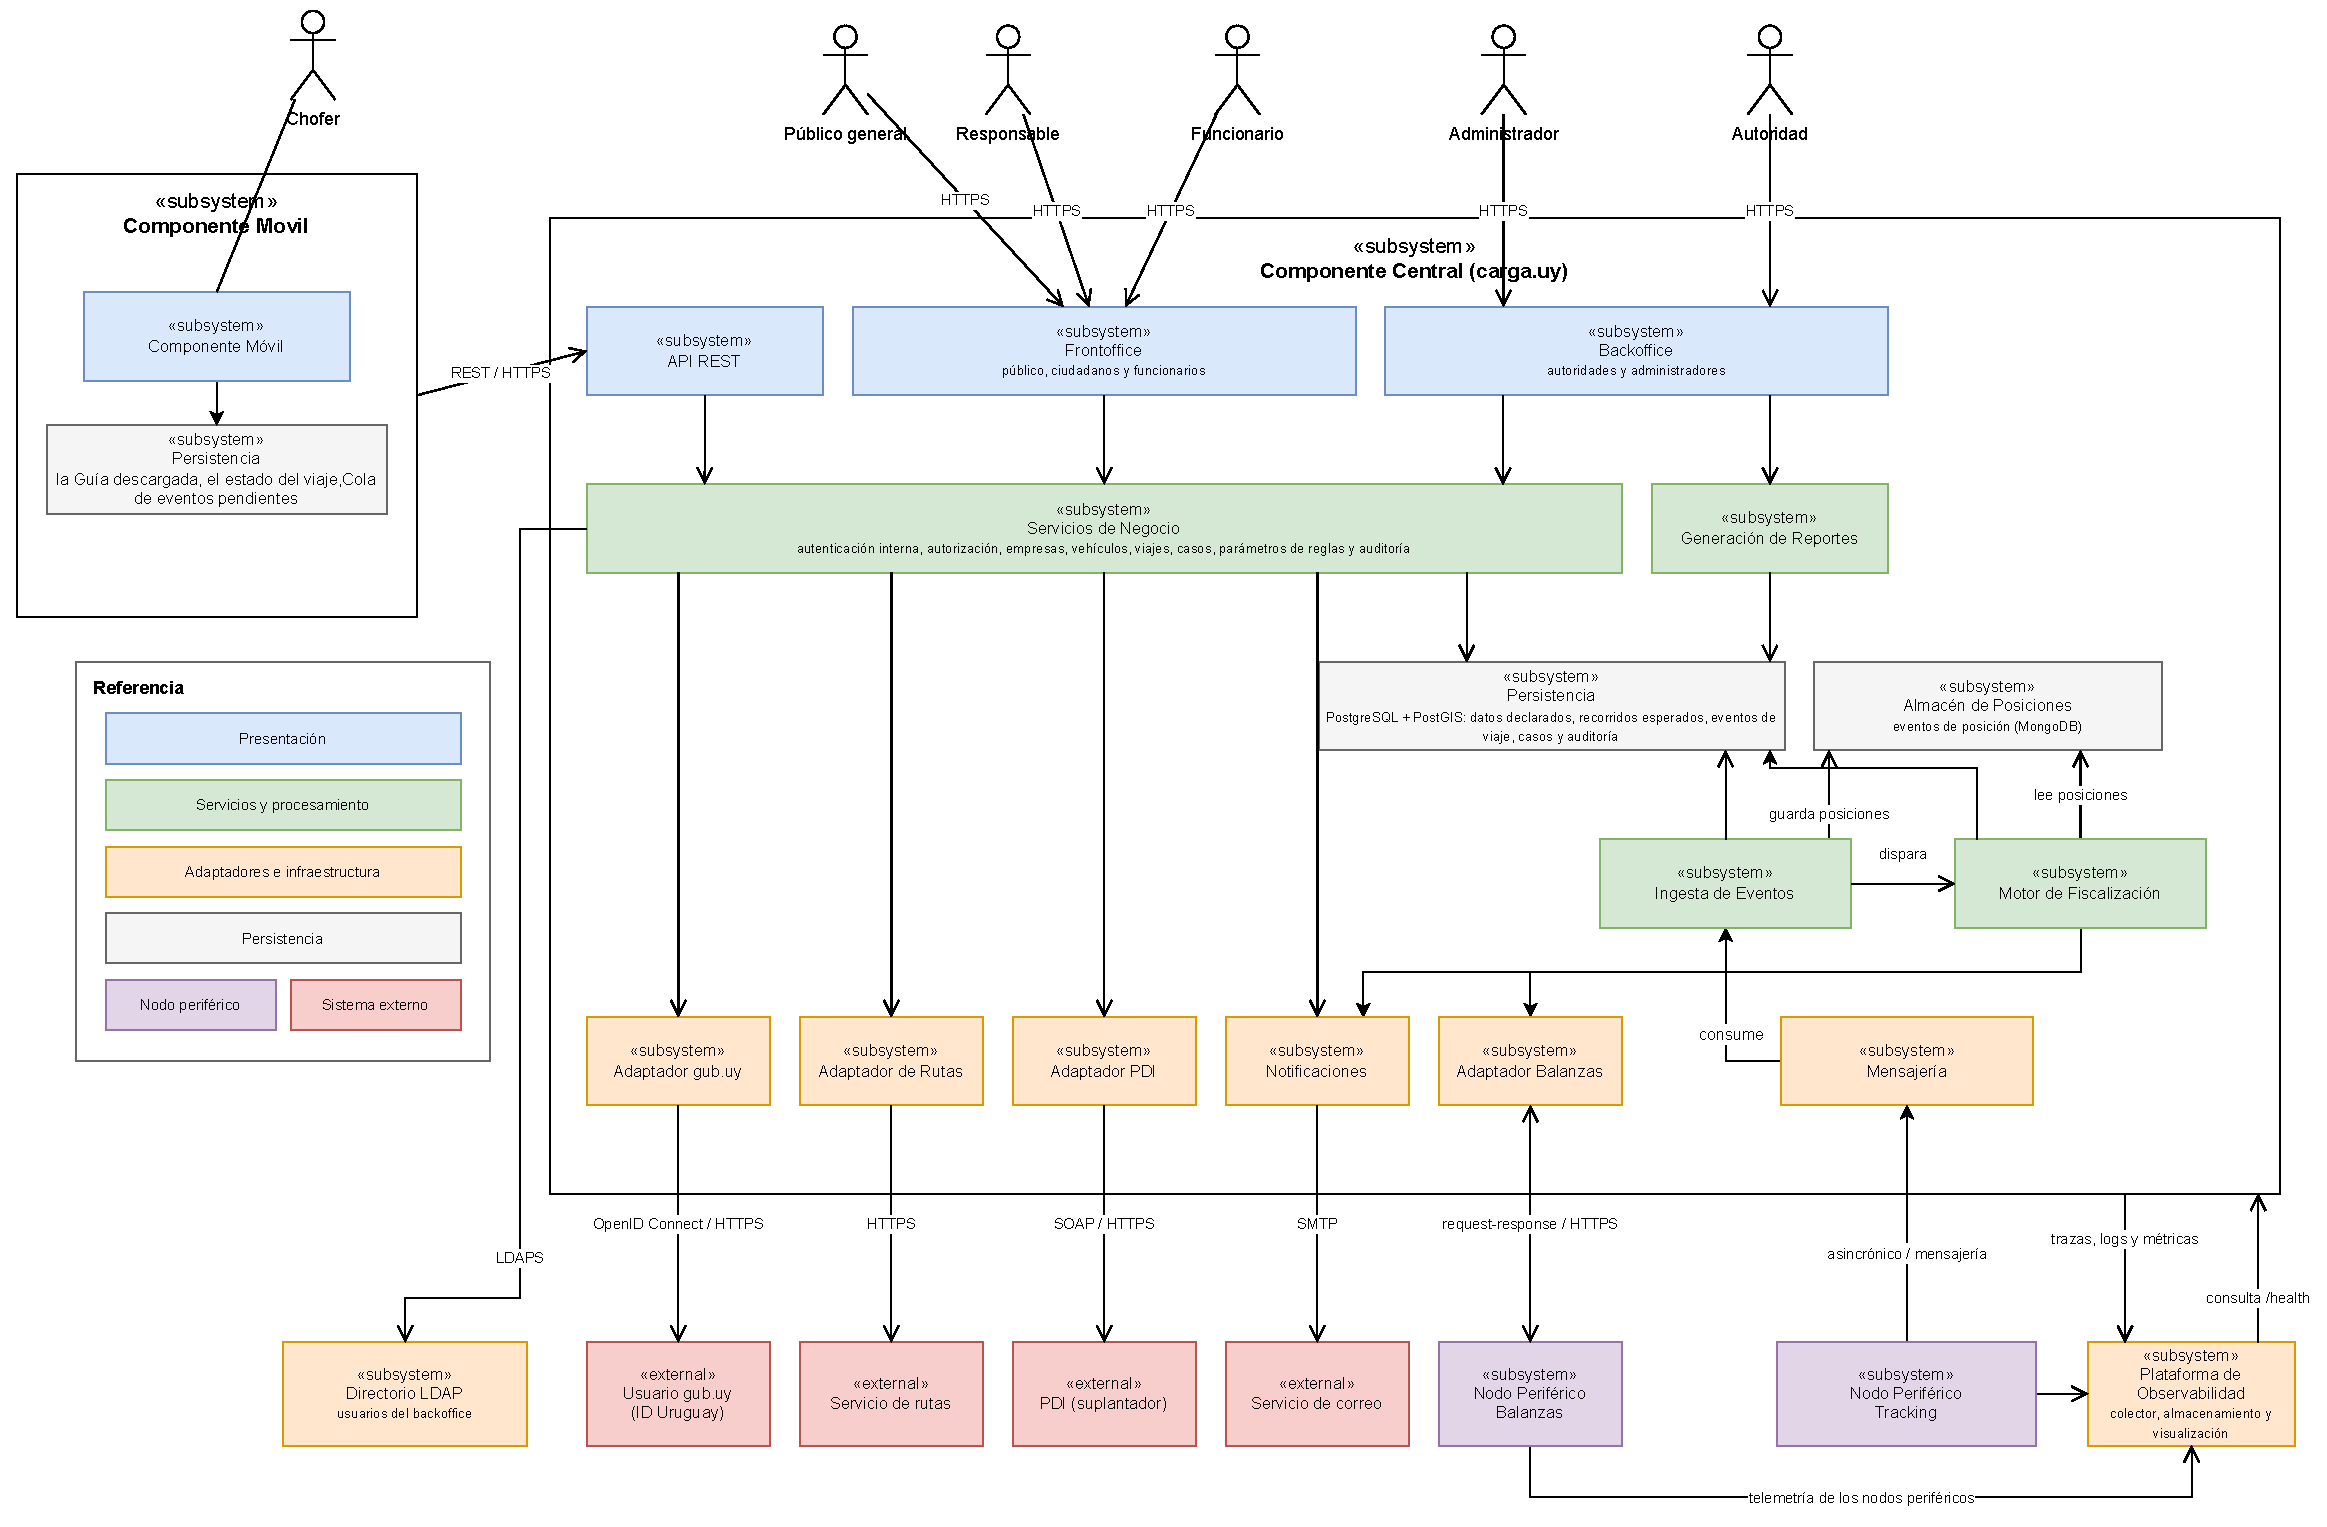
\includegraphics[width=\textwidth]{figures/vista-logica.pdf}
    \caption{Arquitectura general del sistema}
    \label{fig:vista_logica}
\end{figure}

\FloatBarrier

\subsection{Refinamiento 1: Ingesta de Eventos y nodos periféricos}\label{sec:refinamiento-ingesta}

Este refinamiento detalla los subsistemas Mensajería e Ingesta de Eventos, que realizan el CU-10, y el registro de nodos periféricos de los Servicios de Negocio, que realiza el CU-19. La Figura \ref{fig:refinamiento-ingesta} muestra sus componentes, con el clasificador \enquote{component}, y las dependencias entre ellos y con los demás subsistemas de la Figura \ref{fig:vista_logica}. La Tabla \ref{tab:refinamiento-ingesta} describe la responsabilidad de cada componente. Ambas corresponden a lo implementado; el Motor de Fiscalización figura como previsto.

\begin{figure}[H]
    \centering
    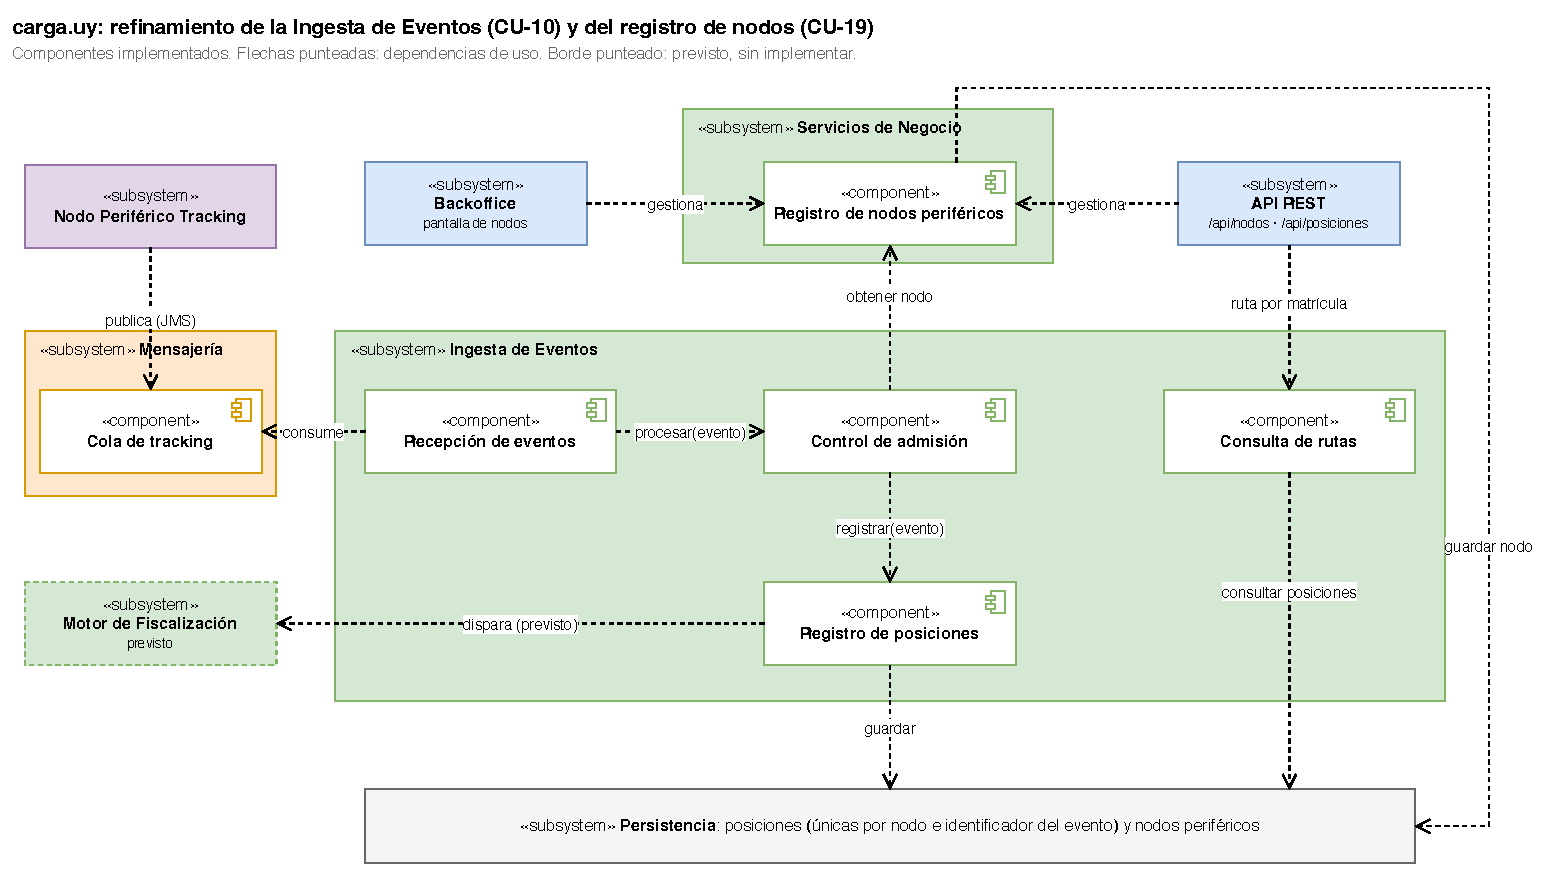
\includegraphics[width=\textwidth]{figures/refinamiento-ingesta.pdf}
    \caption{Vista Lógica, Refinamiento 1: Ingesta de Eventos y nodos periféricos}
    \label{fig:refinamiento-ingesta}
\end{figure}

\begin{table}[H]
    \small
    \centering
    \caption{Componentes de la ingesta de eventos y del registro de nodos}
    \label{tab:refinamiento-ingesta}
    \begin{tabular}{|p{3.6cm}|p{12.2cm}|}
        \hline
        \textbf{Componente} & \textbf{Responsabilidad} \\
        \hline
        Cola de tracking & Recibe los eventos de posición que publica el nodo periférico de tracking. Desacopla la recepción del procesamiento (R4). \\
        \hline
        Recepción de eventos & Consume la cola, interpreta cada evento y descarta los mensajes mal formados. Ante cualquier otra falla deja que el mecanismo de mensajería reentregue el evento. \\
        \hline
        Control de admisión & Acepta solo los eventos de un nodo de tracking registrado y habilitado, que es la precondición del CU-10. \\
        \hline
        Registro de posiciones & Asocia el evento al vehículo por su matrícula y lo almacena. Un evento repetido del mismo nodo choca contra una restricción de unicidad sobre el par (nodo, identificador del evento) y se descarta, lo que hace idempotente la ingesta (R6, AC15). \\
        \hline
        Consulta de rutas & Devuelve las posiciones de un vehículo ordenadas por su momento de generación y no por el orden de llegada (AC16). \\
        \hline
        Registro de nodos periféricos & Mantiene los nodos de balanzas y de tracking con su tipo, punto de acceso y estado. Todo nodo nuevo queda deshabilitado; cambiar su punto de acceso lo vuelve a deshabilitar; la baja es lógica (CU-19). \\
        \hline
    \end{tabular}
\end{table}

\pendiente{agregar los refinamientos de los demás subsistemas que el grupo considere necesarios, por ejemplo los Servicios de Negocio o el Motor de Fiscalización.}

\FloatBarrier

\subsection{Diagramas de Interacción}

En esta sección se incluyen diagramas de secuencia UML, a nivel de componentes, vinculados a los casos de uso críticos que se consideró necesario especificar con mayor detalle.

\subsubsection{CU-10 Ingerir y procesar eventos de tracking}\label{sec:interaccion-cu10}

La Figura \ref{fig:secuencia-cu10} muestra la interacción para el CU-10, de acuerdo con el refinamiento de la Sección \ref{sec:refinamiento-ingesta}. El nodo periférico de tracking publica el evento en la Mensajería, que lo entrega a la Ingesta de Eventos de forma asincrónica. Un mensaje mal formado se descarta sin reintento. La ingesta solo continúa si el evento proviene de un nodo de tracking registrado y habilitado; en ese caso obtiene el vehículo por su matrícula y registra el evento. Si el par (nodo, identificador del evento) ya estaba registrado, la restricción de unicidad lo rechaza y el evento se descarta como duplicado. Si es nuevo, se asocia al viaje que estaba en curso cuando se generó (Sección \ref{sec:cu-10}), se dispara el Motor de Fiscalización (Sección \ref{sec:interaccion-cu11}) y se actualizan las métricas. El orden de la ruta se reconstruye al consultarla, por el momento de generación de cada evento.

\begin{figure}[H]
    \centering
    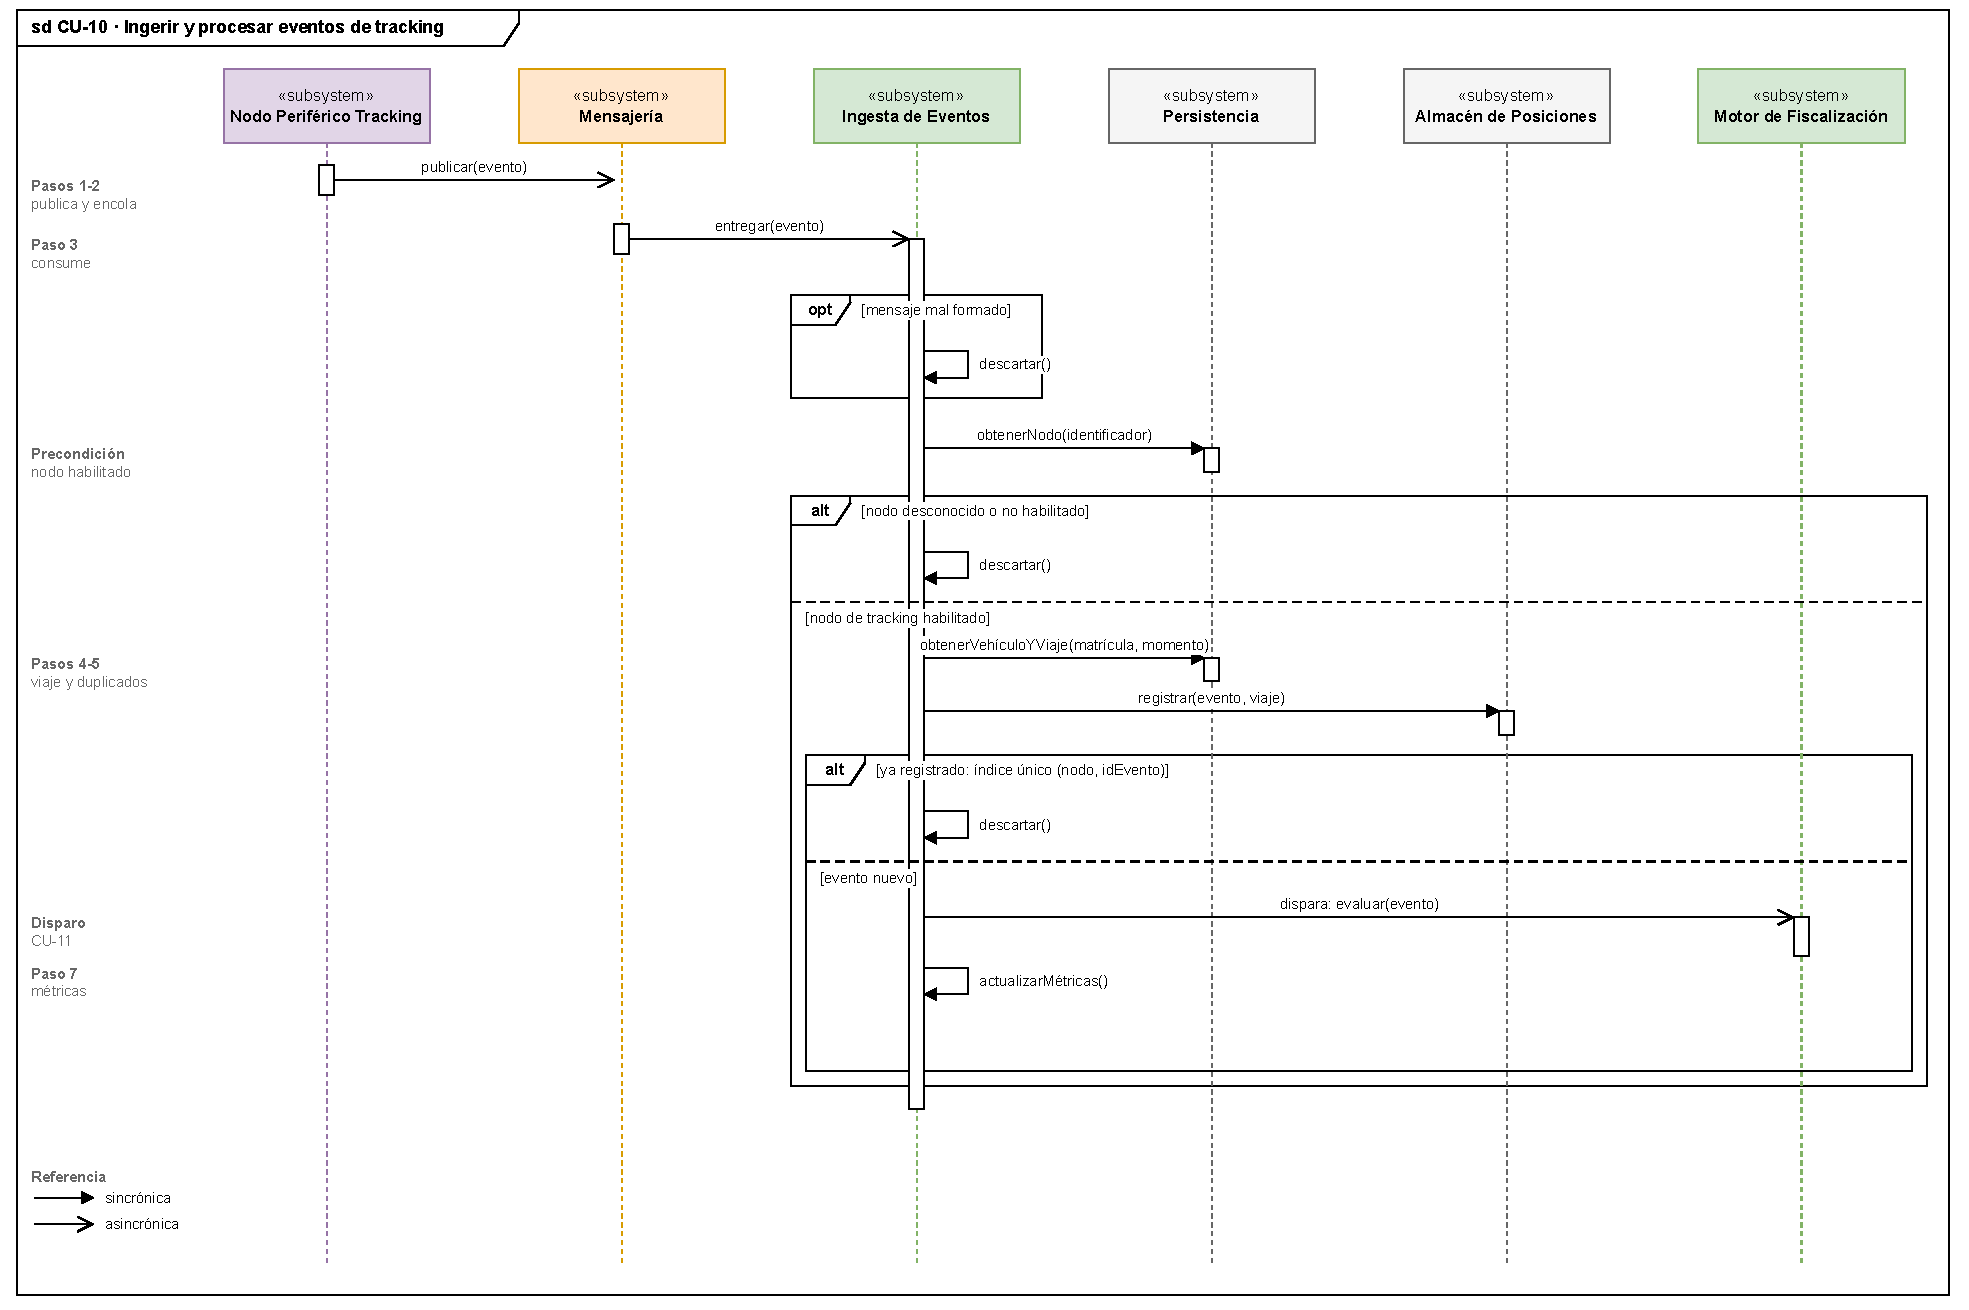
\includegraphics[width=\textwidth]{figures/secuencia-cu10.pdf}
    \caption{Diagrama de secuencia del CU-10}
    \label{fig:secuencia-cu10}
\end{figure}

\FloatBarrier

\subsubsection{CU-11 Detectar automáticamente un incumplimiento y generar el caso}\label{sec:interaccion-cu11}

La Figura \ref{fig:secuencia-cu11} muestra la interacción entre los componentes de la vista lógica para el CU-11. Comienza cuando la Ingesta de Eventos, al terminar el procesamiento del CU-10, dispara de forma asincrónica al Motor de Fiscalización. El fin de un viaje registrado desde el móvil (CU-09) dispara el mismo flujo. El motor evalúa las cuatro reglas de la Sección \ref{sec:vista-casos-de-uso}: exceso de carga, consultando los pesajes al nodo de Balanzas solo cuando el evento es el fin de un viaje (DA10); vigencia del Permiso y la ITV; viaje sin Guía; y desvío de ruta, contra el recorrido esperado y los umbrales parametrizados. Si detecta un incumplimiento, verifica que el hecho no haya generado otro caso; si no existe, crea el caso con su evidencia, notifica a la empresa, inicia el plazo de descargo y registra la creación en la pista de auditoría. Los pasos y las alternativas siguen la ficha del CU-11.

La notificación a la empresa es asincrónica: el motor le pide el aviso al subsistema de Notificaciones y continúa, para que una falla del correo no bloquee la creación del caso. El caso pasa a \emph{notificada}, y comienza el plazo de descargo, recién cuando el servidor de correo acepta el envío. Si el envío falla, Notificaciones lo reintenta y el caso permanece en \emph{detectada}, de modo que a la empresa no se le cuenta el plazo de un aviso que todavía no recibió. La creación del caso se registra en la pista de auditoría al final, como indica la ficha del CU-11.

\begin{figure}[H]
    \centering
    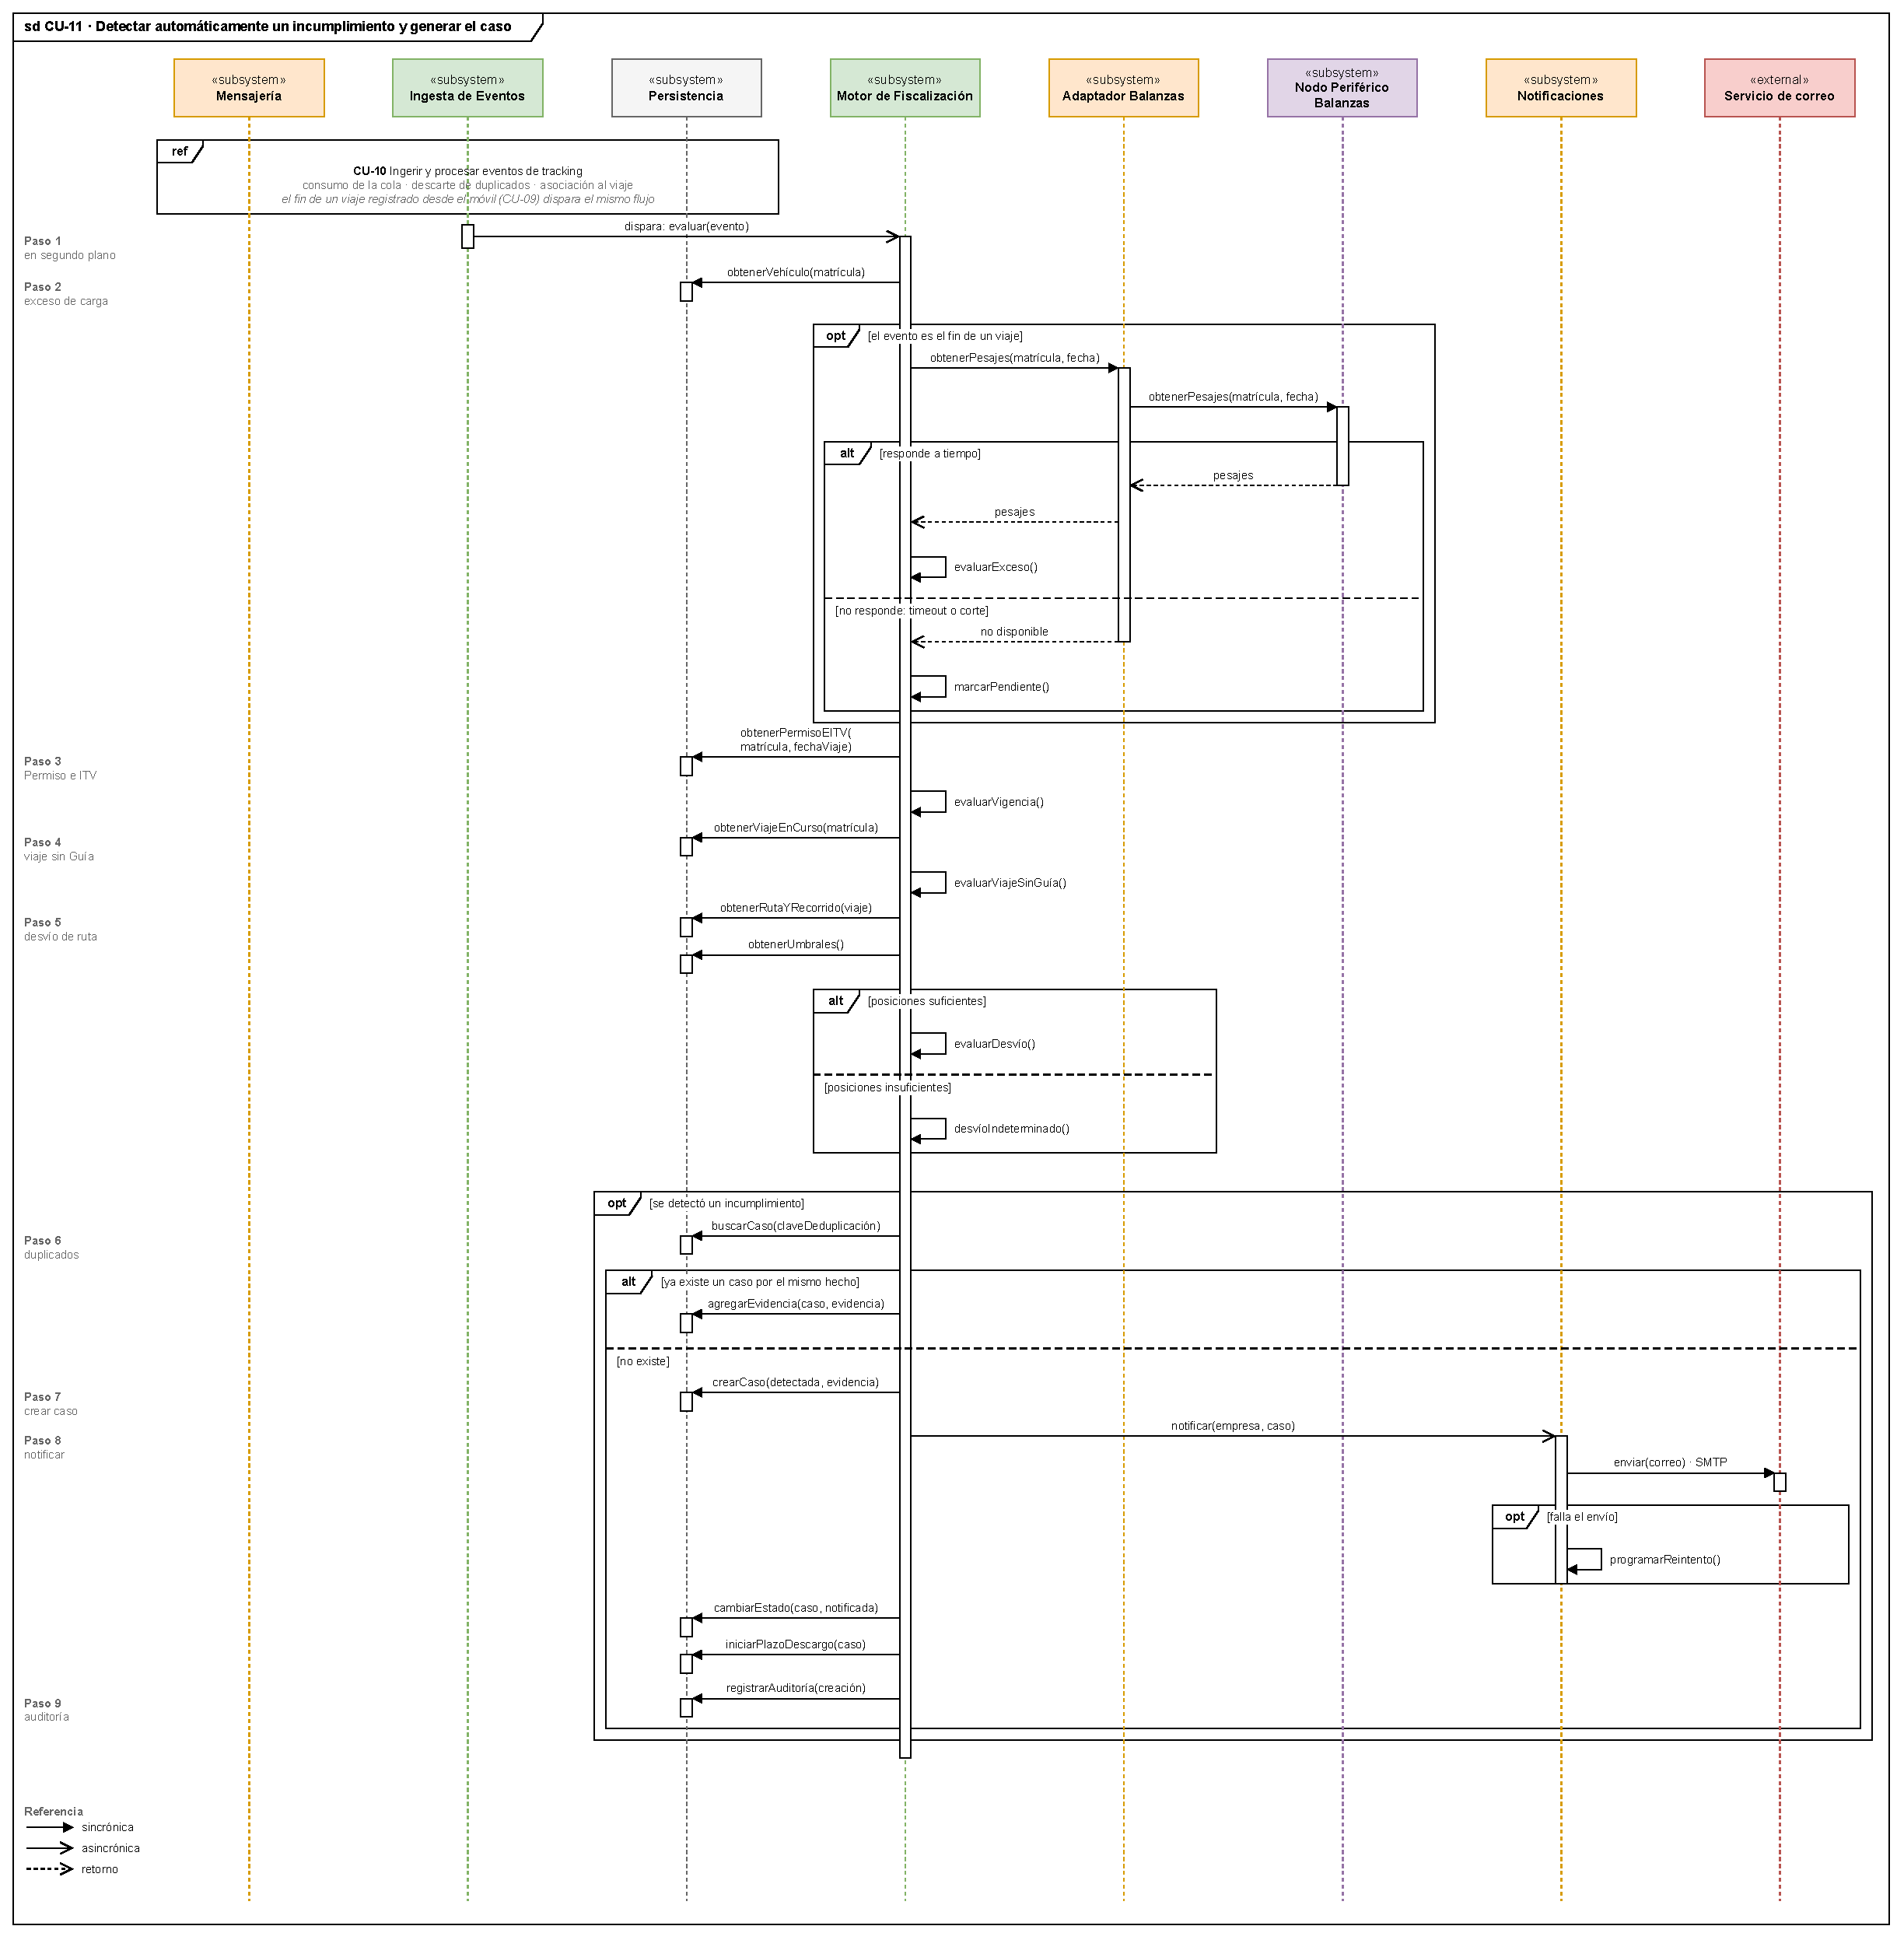
\includegraphics[width=\textwidth]{figures/secuencia-cu11.pdf}
    \caption{Diagrama de secuencia del CU-11}
    \label{fig:secuencia-cu11}
\end{figure}

\FloatBarrier
